\versoquote{\raisebox{-1.5em}{\resizebox{!}{2.15em}{\includestandalone{figures/qabuum}}}}{\raisebox{-0.7em}{\resizebox{!}{1.7em}{\includestandalone{figures/emegir}}}}
%You are not one who stays in one place, you are one who is everywhere. --Sumerian Saying
\chapter[Delocalised Oxygen TLSs In Low Dimensions][TLSs In Low Dimensions]{Delocalised Oxygen TLSs In Low Dimensions}\label{ch:tlslow}
\lofchap{Delocalised Oxygen TLSs In Low Dimensions}
\chapterprecis{Investigating the effects of local potential perturbations on an oxygen atom. Calculation of candidate TLS properties such as $E_{01}$ energy splitting and dipole moments.  }

\thought{Equipped with a framework describing} the behaviour of an oxygen atom delocalising in the presence of an external potential, we are now in a position to investigate which atomic configurations may demonstrate TLS characteristics.
Whilst other properties have been measured, we will focus on obtaining respectable values for $E_{01}$ and dipole strength, assuming our model defect is embedded inside a fictitious phase qubit.
Expected values are approximately $E_{01}=8$ GHz and $\wp=1.2$ $e$\AA~\cite{Cole2010}.
This will enable us to directly compare measured qubit-TLS couplings via \cref{eq:smax} to our calculated splitting energies and dipole values.

Starting with the model outlined in \cref{ch:tise}, \cref{sec:methdipole} extends these methods to treat oxygen delocalisation in two dimensions, and introduces an expression to calculate the effective dipole of the oxygen relative to an external field.
\Crefrange{sec:bonds}{sec:tls} begin with a minimal example of this model and slowly add complexity, so interactions can be examined and understood in a systematic way.
\Cref{sec:bonds} considers a defect comprising of an Al--O--Al chain in one dimension, perturbed from a crystalline lattice, simulating defects A and B in \cref{fig:sio2}.
In reality, an oxygen atom in the amorphous layer of a Josephson junction will be surrounded by atoms in all three dimensions (which can be expressed using a cluster of atoms simulated in \cref{ch:junctions}).
Moving towards a model representation of this, \cref{sec:2d} extends the model to two dimensions, with four aluminium atoms confining an oxygen in a plane.

\section[\lin{2D} Formalism and Dipole Expression]{2D Formalism and Dipole Expression}\label{sec:methdipole}

To extend the Hamiltonian $H$ \cref{eq:OHam} into a two dimensional matrix representation, one must arrange data in a way which is understood by the \sw{eigs} function, which expects a two dimensional sparse matrix.

If $\mathbf{r}=(x,y)$ in \cref{eq:tisemat}, we can treat each dimension separately and follow the method outlined in \cref{sec:methdipole} for $x$ then $y$.
With two sparse matricies, the Kronecker product can be applied to generate a block matrix ready for diagonalisation.
\begin{equation}
H = H_x \otimes \mathbb{I}_y + \mathbb{I}_x \otimes H_y.
\label{eq:h2d}
\end{equation}

The dipole element is computed using numerical integration of the ground- and first-excited states ($\psi_0$, $\psi_1$), where
\begin{equation}
    \wp_x = \iint \psi_0^*(x,y) x \psi_1(x,y) \,\mathrm{d}x\mathrm{d}y
    \label{eq:dipole}
\end{equation}
is an example of the dipole in the $x$ direction.\nomref{BP}{eq:dipole}

Relative differences in energy levels (\ie energy splittings) are an important measure of the model.
We therefore define a convention where $E_{ij} = E_j-E_i$, such that the ground state ($E_0$) to first excited state ($E_1$) energy splitting is defined as $E_{01}$.
For comparison with experimental results, energy is expressed in frequency units throughout this discussion.\nomref{Z01}{sec:methdipole}

\section[TLSs as Perturbed Bond Angles]{TLS Defects as Perturbed Bond Angles in a Lattice}\label{sec:bonds}

Consider the two simplest cases in \cref{fig:sio2}: defect type A; where the aluminium--oxygen bond distance is shortened, forcing the oxygen to occupy two off axis positions, and defect type B; where the opposite occurs: the aluminium--oxygen bond distance is lengthened, allowing two preferred oxygen positions on axis.

These two defect types can be modelled by solving our system Hamiltonian \cref{eq:OHam} for three atoms: an oxygen with two aluminium atoms at a lattice coordinate apart, displaced toward and away from the oxygen.
For example, corundum has an Al--O bond distance of $\sim\!1.85$ \AA.
If we define the oxygen position to be at an origin, the aluminium atoms can be considered as pairs ($x = -X, \: +X$ = \{$\pm 1.85$ \AA\}) lying on a cardinal axes; which are identified henceforth as $\abs{X}$ or simply the \textit{defect pair}.
Displacing $\abs{X}$ equidistantly from this origin (\ie moving away from optimal crystalline configuration) will yield either an A or B type defect, depending on the direction of displacement.\nomdref{Babs}{$\abs{\cdot}$}{A pair of atoms displaced equidistantly from an origin, \eg $\abs{X} = -X, \: +X$}{sec:bonds}

An eigenspectrum of the six lowest energy levels of this system over a continuum of values in $\abs{X}$  is depicted in \cref{fig:spectrum}.
Each energy is measured relative to the ground state, which shows two particular regions where $E_{01}$ (green, solid line) is degenerate (labelled sections A and B: both associated with the respective defect type).
There exists a third (an)harmonic region (section C), which reaches a harmonic state at a separation distance of $\abs{X} \sim 1.85$ \AA: the optimal corundum Al--O bond distance.
At this distance the spatial harmonic approximation holds and the oxygen can be considered to be localised.

\begin{figure}[htp]
  \resizebox{0.9\textwidth}{!}{\includestandalone{figures/eigenspectrum}}
  \caption[Three Atom Eigenspectrum]{\label{fig:spectrum}Eigenspectrum of a three atom system Al--O--Al, over a varying distance separation. Each excited state has been normalised with the ground state, which shows two regions with a degeneracy at the lowest level. Section A is indicative of the A type defect (\cref{fig:Atype}), section B of the B type (\cref{fig:Btype}). An (an)harmonic crossover point is also extant, labelled as section C, which is approximately centered about the optimal Al--O bond distance of corundum ($1.85$ \AA).}
\end{figure}

To investigate the potential landscape and the resultant oxygen wavefunction in sections A and B of \cref{fig:spectrum}, we choose two separation distances: $\abs{X} = 1.5$ \AA\ (\cref{fig:Atype}), which lies in the A type defect section, and $\abs{X} = 2.2$ \AA\ (\cref{fig:Btype}), which exists in the B type defect section.
Although the Al--O--Al chain is arranged in a line, we consider delocalisation of the oxygen in two dimensions so that both defect types can be identified on a continuum separation in $\abs{X}$ (as \cref{fig:spectrum} depicts) rather than using two separate coordinate systems.

\begin{figure}[htp]
\resizebox{\textwidth}{!}{\includestandalone{figures/atype}}
\caption[A Type Ground State Wavefunction]{\label{fig:Atype}A top down view of the potential seen by an oxygen atom with two aluminium atoms closer than an appropriate lattice distance (truncated at $0$ eV, gray). The ground state eigenmode of the oxygen can be seen in the center (green/yellow). This configuration has a separation distance of $\abs{X} = 1.5$ \AA\ and is representative of an A type defect (see \cref{fig:sio2}). \lin{1D} potential values and projected wavefunctions, which are anchored to the ground state energy \plotline{line width=0.75pt,color=gray!50} are plotted in the outsets to better indicate the depth of the potential well.}
\end{figure}

\begin{figure}[htp]
\resizebox{\textwidth}{!}{\includestandalone{figures/btype}}
\caption[B Type Ground State Wavefunction]{\label{fig:Btype}A top down view of the potential seen by an oxygen atom with two aluminium atoms further apart than an appropriate lattice distance (truncated at $0$ eV, gray). The ground state eigenmode of the oxygen can be seen in the center (green/yellow). This configuration has a separation distance of $\abs{X} = 2.2$ \AA\ and is representative of a B type defect (see \cref{fig:sio2}).  \lin{1D} potential values and projected wavefunctions, which are anchored to the ground state energy \plotline{line width=0.75pt,color=gray!50} are plotted in the outsets to better indicate the depth of the potential well.}
\end{figure}

Both figures show a top down view of the potential exerted on the oxygen by the two aluminium atoms (gray), whose positions lie at the centre of the circles.
We truncate potential energy values above $0$ eV for clarity, where energy is measured relative to the zero point set by the Streitz-Mintmire potential's electronegativity correction. The ground state wavefunction (green/yellow) indicates the spatial probability of the oxygen atom in these configurations.
It can be seen in \cref{fig:Btype}, where the pair is far apart, two local minima exist in the form of rings around the base of each aluminium position.

Equivalences between the A and B type defects illustrated in \cref{fig:sio2} are clearly visible: \cref{fig:Atype} showing a shortened bond length, causing an oxygen dipole perpendicular to the bond axis, and \cref{fig:Btype} depicting a lengthened bond and an oxygen dipole parallel to the bond axis.

The functional form of the \lin{1D} potential (outset axes of \cref{fig:Atype,fig:Btype}, \plotline{line width=1.25pt}; either $V(x,0)$ or $V(0,y)$) in the direction of the defect is a double well.
Also depicted in these outsets are projected wavefunctions, which have been scaled for visual purposes, but anchored at the ground state energy \plotline{line width=0.75pt,color=gray!50}.
This representation is equivalent to the standard two level physics depiction of the TLS, and as such, potential offsets $\epsilon$ and tunneling matrix elements $\Delta$ (see \cref{sec:glass}) of our model may be estimated in this limit.

\section{TLS Defect Confined in Two Dimensions}\label{sec:2d}

The ideal case discussed in \cref{sec:bonds} ignores many real world complications, in particular any potential constraints from nearest neighbour atoms that undoubtedly surround the TLS.
In an attempt to add complexity to the model gradually, we start with two additional aluminium atoms on the same plane as \cref{fig:Atype,fig:Btype}, confining the defect in the $\abs{Y}$ direction (\ie $y = -Y, \: +Y$).

Throughout the discussion we use the term \textit{defect pair} to refer to the pair of aluminium atoms which provide the dominant contribution to the potential felt be the oxygen.
The term \textit{confining pair} in contrast is used to refer to additional neighbouring aluminium atoms which also apply major influence to perturb the symmetries of the potential.

\section{Classifying Eigenspectrum Dynamics}\label{sec:dynamics}

As the values of $\abs{X}$ or $\abs{Y}$ are altered, a complex interplay between the excited states of the model can result.
Simple two-level degeneracy and harmonic states are no longer the only possibilities. To interpret what is occurring in a certain domain, we define a metric using the ground and four lowest excited state energies
\begin{equation}
\xi=\frac{E_{1}-E_{0}}{E_{2}-E_{0}}+\frac{E_{3}-E_{0}}{E_{4}-E_{0}}.
\label{eq:ximetric}
\end{equation}
This metric ranges from $0$ to $2$ and can give a qualitative understanding of the eigenspectrum of the defect.\nomdref{Gxi}{$\xi$}{$\xi$ metric: a qualitative expression used to interpret eigenspectra}{eq:ximetric}
To understand why this is useful, we need first to consider the new symmetries which are possible in a \lin{2D} potential.

To begin we generate a phase space diagram where $\xi$ is plotted as a function of the distance to the confining aluminium atoms ($\abs{X},\abs{Y}$).
Each phase diagram is split into at least four domains, where the properties of these domains can be explained through the interplay of potential configuration and dipole alignment (discussed in \cref{sec:dipole}).
Focusing for now on the influence of potential shape, the \lin{2D} potential can be approximated as two \lin{1D} potentials: one projected in the $x$ direction and the other along $y$.
A simple harmonic potential in \lin{2D} is quadratic in both $x$ and $y$.
However, for TLS physics there are two relevant configurations: a set of two double wells (tetra-well) or a set of a double and harmonic well (hemi-tetra-well); which are both illustrated in \cref{fig:mexhatproj}.
It is clear from the outset potential projections of \cref{fig:Atype,fig:Btype} that both A and B type defects reside in hemi-tetra-wells.

\begin{figure}[htp]
\resizebox{0.8\textwidth}{!}{\includestandalone{figures/mexhatproj}}
\caption[Potential Projections]{\label{fig:mexhatproj}\lin{1D} double wells \plotline{line width=1.5pt,color=Set1-5-2} and harmonic wells \plotline{line width=1.5pt,dashed,color=Set1-5-1} can be used to represent simple projections of a \lin{2D} potential onto the $x$ and $y$ axes. Left: two projected double wells is an example of a tetra-well. Right: a combination of one double well and a harmonic well reflects the hemi-tetra- case.}
\end{figure}

The $\xi$ metric is capable of identifying the tetra- ($\xi=0$) and hemi-tetra- ($\xi=1/2$) domains, as well as harmonic ($\xi=5/4$) and unique ground state (rotationally symmetric, Mexican hat-like) ($\xi=2$) regimes and finally the location of bifurcations or transitions ($\xi=1$).
\Cref{fig:ximetric} shows the corresponding layouts of each interplay.
It is worth noting that $\xi=3/2$ can also be considered harmonic for the lowest three levels.

\begin{figure}[htp]
  \resizebox{\textwidth}{!}{\includestandalone{figures/ximetric}}
  \caption[$\xi$ Metric]{\label{fig:ximetric}Energy level representation of the lowest five eigenenergies of a candidate defect and their associated $\xi$ value. $\xi=0$: the tetra-well domain, $\xi=1/2$: the hemi-tetra-well domain, $\xi=5/4$: the harmonic region and $\xi=2$: the unique ground state region. The bifurcation/transition region, $\xi=1$ is not clearly defined thus an example is not shown here.}
\end{figure}

\section{Visualising Phase Space and Identifying TLSs}\label{sec:phasespace}

Using this $\xi$ metric and varying the values of both $\abs{X}$ and $\abs{Y}$ generates \cref{fig:xiunbound}, a phase map of the interplay of low energy states of the oxygen atom confined in two dimensions by aluminium atoms.
The $x$ and $y$ axes show the $\abs{X}$ and $\abs{Y}$ pair separation distances respectively over a range of $1.85\!-\!4$ \AA\ and the phase colour indicates which $\xi$ region a particular configuration exists in.

\begin{figure}[htp]
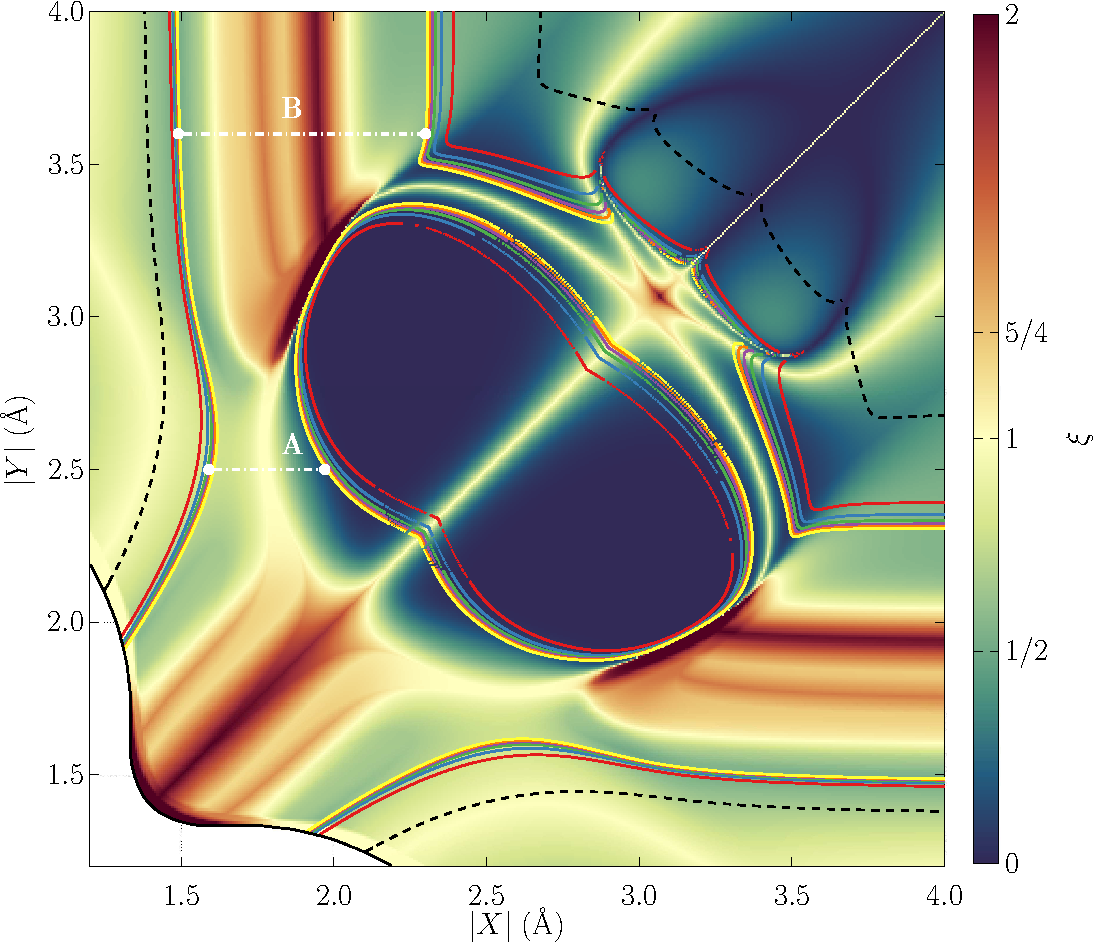
\includegraphics[width=\textwidth]{figures/xiunbound}\\
\caption[$\xi$ Metric Phase Map, Unbound in $z$]{\label{fig:xiunbound}Map of the $\xi$ metric of the delocalized oxygen \lin{2D} model. The $\abs{X}$ and $\abs{Y}$ axes represent aluminium pair position separations. \plotline{line width=1.5pt,dashed} represents a minimum resolvable energy splitting of $10$ kHz. The white (blank) section indicates where the aluminium atoms are so close, the oxygen confinement region no longer exists. Overlayed contour lines corresponding to $E_{01} = 0.5\!-\!10$ GHz (red to yellow) are comparable to existing experimental qubit results. Cases where quad-degeneracy exists are denoted as dotted rather than solid contours. Two traces (white, dash-dotted lines) are also depicted. The first, at $\abs{Y} = 2.5$ \AA\ (labelled A) is plotted in \cref{fig:tetraspectrum}. In contrast, the trace at $\abs{Y} = 3.6$ \AA\ (labelled B) yields an equivalent eigenspectrum to the \lin{1D} case in \cref{fig:spectrum}.}
%\plotline{thin,double distance=2pt,dash dot}
\end{figure}

Regions that are deemed to be unimportant when searching for TLS behaviour are those where $\xi \geq 1$, as these correspond to eigenspectra which do not possess a doubly degenerate ground state.

As discussed in \cref{sec:bonds}, in the one dimensional confinement case, both A and B type defects exist in a hemi-tetra-well ($\xi = 1/2$).
This is also the case for the two dimensional landscape---contour lines corresponding to $E_{01} = \{0.5, 2, 4, 6, 8, 10\}$ GHz (red--yellow) on \cref{fig:xiunbound} show the configuration properties that result in TLS $E_{01}$ splittings in qubit architectures described in \cref{sec:phenom}.
For example: anywhere an orange, $8$ GHz line exists on this phase map, the $\abs{X}, \abs{Y}$ coordinates of the model generate a cluster configuration that yields the same $E_{01}$ observed in phase qubit experiments~\cite{Cole2010}.

Many of these lines lie completely within a $\xi = 1/2$ (green) region.
Consider the contour set on the left of \cref{fig:xiunbound} where $\abs{X} \simeq 1.5$ \AA: \Cref{sec:bonds} states this distance is indicative of an A type defect.
The addition of the $\abs{Y}$ aluminium pair does little to perturb the potential at larger distances ($\abs{Y} \gtrsim 3$ \AA) and causes only slight deformations at smaller distances ($2 \lesssim \abs{Y} \lesssim 3$ \AA).
As the phase space is symmetric about $\abs{X} = \abs{Y}$, A type defects exist at the bottom of the plot where $\abs{Y} \simeq 1.5$ \AA\ as well.

B type defects also exist in a $\xi = 1/2$ region, when $\abs{X}$ or $\abs{Y} \simeq 2.4$ \AA.
The orthogonal pair separation distance is at least $1$ \AA\ larger than the defect pair in these configurations and therefore have no bearing on the potential seen by the oxygen.
Complications arise when the orthogonal pair is closer and begins to confine the defect.
To explain this response, a better understanding of the domains of the map is required.

\section{Analysis of Phase Space Domains}\label{sec:phaseanalysis}

The case of $\xi = 0$ is particularly interesting in this scenario: a tetra-well region, causing a quad degeneracy in the ground state.
In this region, the characteristics of a B type defect are strongly modified.
To understand why, we first explain the large rounded $\xi = 0$ domains in the centre of \cref{fig:xiunbound}'s phase space.

Tetra-well domains exist when the confinement potential acting on the oxygen consists of two double wells (see left plot in \cref{fig:mexhatproj}).
This phenomena emerges when both the defect pair and the confining pair of atoms are close enough to interact.
Consider an A type defect with a defect pair in $\abs{X}$ and a confining pair at a constant value of $\abs{Y} = 2.5$ \AA.
If $\abs{X}$ is varied from an initial value of $1.6$ \AA\ to $2$ \AA, this extension spans phase space from one point where $E_{01} = 8$ GHz to another.
This separation is traced on \cref{fig:xiunbound} (white dash-dotted line labelled A), where the defect visibly moves from a hemi-tetra- regime ($\xi = 1/2$) and goes through a transition region before reaching the tetra-well regime ($\xi = 0$).
\Cref{fig:tetraspectrum} depicts the eigenspectrum of this trace.
This is in contrast to larger confining pair values such as $\abs{Y} = 3.6$ \AA\ (also traced on \cref{fig:xiunbound}: white dash-dotted line labelled B) where the eiginspectrum is largely unchanged from the one dimensional case presented in \cref{fig:spectrum}.

\begin{figure}[htp]
  \resizebox{0.9\textwidth}{!}{\includestandalone{figures/tetraeigspect}}
  \caption[Eigenspectrum of a \lin{2D} TLS]{\label{fig:tetraspectrum}Eigenspectrum of a \lin{2D} TLS: an oxygen atom caged with four aluminum atoms. Each excited state has been normalised with the ground state. The confinment pair $\abs{Y}$ is held at a constant distance separation of $2.5$ \AA\ and the $\abs{X}$ range shows how higher eigenvalues behave as the confinement atoms force the defect into a tetra-well regime. \Cref{fig:xiunbound} depicts this data in terms of $\xi$ (white dash-dotted trace labelled A). }
\end{figure}

As the $\abs{X}$ separation distance is increased, the effect on $E_{01}$ is negligible on the scale of the higher energy levels (although differs greatly on the TLS splitting energy scale).
However, the degenerate pair $E_{23}$ (a degenerate second and third excited state pair) rapidly shifts from a level much higher than ground to degenerate at ground.
Complete quad-degeneracy is not always extant in the tera-well regime, configurations of $\abs{X}$ and $\abs{Y}$ in these domains usually have two degenerate pairs which are still observable, akin to the hemi-tetra- domains, with the difference \textit{between} the pairs approaching the difference \textit{of} the pairs: $E_{01} = E_{23} \approx E_{12}$ ($1.95 \lesssim \abs{X} \leq 2$ \AA\ in \cref{fig:tetraspectrum} for example).
In other words, when the ground to first excited and second to third excited state differences are equal, the first to second excited state difference trends from a much larger value to one effectively equivalent to the aforementioned pairs in this region.

When considering the influence of higher lying excited states, it's important to keep the fundamental energy scales of the problem in mind.
In typical qubit experiments, the superconducting properties of the device put a rigorous upper limit on TLS frequencies of interest.
At frequencies greater than approximately $100$ GHz, there is enough energy to dissociate Cooper-pairs and therefore it can be viewed as an operational upper bound for Josephson junction devices (typical operating frequencies are however device specific, and are much lower in practice).
For much of the tetra-well domain $E_{12} \geq 100$ GHz and consequently can effectively be ignored, the system can be considered as a two-level defect even in this quad degeneracy domain.

The B type defects' sudden behaviour change as $\abs{X}\rightarrow\abs{Y}$ is also caused by this response (see \cref{fig:xiunbound}).
Confinement pairs start interacting with the defect, causing $E_{23}$ to approach the value of $E_{01}$ (again, $1.95 \lesssim \abs{X} \leq 2$ \AA\ in \cref{fig:tetraspectrum} depicts this phenomena).
The $\xi$ metric does not clearly differentiate between two degenerate pairs that are marginally separated and two pairs that are actually degenerate.

If however, $E_{12} < 100$ GHz, higher lying energy states must still be considered and the model exhibits true quad degenerate behaviour.
Regions in which this occurs are denoted in \cref{fig:xiunbound} as dotted contours, which over the entirety of phase space are extremely rare---suggesting a reason why quad-level systems are yet to be experimentally observed.

The final domain yet to be discussed on \cref{fig:xiunbound} is the upper right hand corner where both $\abs{X}$ and $\abs{Y}$ are large.
This region is tetra-well dominated but can be considered as a region where the TLS model breaks down.
Each of the four potential minima exist localised about the four confining aluminium atoms and as such should not be considered as TLS candidates.

\section{Chapter Summary}

The number of possible atomic configurations in an amorphous structure is immense.
Even within an ultra-thin barrier such as the JJ oxide layer, the state space is still vast.
Before investigating even a small subset of these possibilities, this chapter shows that analysis of local variations at the nearest neighbour level provides an abundance of useful information an oxygens properties.

Understanding how the eigenspectrum of an oxygen atom responds in the presence of an external potential in this comprehensive manner allows us, in \cref{ch:tlsphase}, to compare calculated TLS properties from this model to measurements obtained from experiments.    